 % !TEX encoding = UTF-8 Unicode
% !TeX TXS-program:compile = txs:///pdflatex/[--shell-escape] 

\documentclass[12pt, twoside]{book}
%***************************************************************************************************

% Podstawowe ustawienia języka, według którego formatowany będzie dokument
%\usepackage[english,polish]{babel}
\usepackage[english]{babel}

% Pakiet babel dla polskiego języka powoduje konflikt z pakietem amssymb.
% Polecenie '\lll' definiują oba pakiety - porządana jest druga definicja.
\let\lll\undefined

% W przypadku wielojęzykowości ustawia główny język dokumentu
\selectlanguage{english}

% Kodowanie dokumentu
\usepackage[utf8]{inputenc} 
\usepackage[T1]{fontenc} 

% Dowolny rozmiar czcionek, kodowanie znaków
\usepackage{lmodern}

% Polskie wcięcia akapitów
\usepackage{indentfirst}

% Polskie formatowanie typograficzne
\frenchspacing

% Zapewnia liczne usprawnienia wyświetlania i organizacji matematycznych formuł. 
\usepackage{amsmath}

% Wprowadza rozszerzony zestaw symboli m.in. \leadsto
\usepackage{amssymb}

% Dodatkowa, ,,kręcona'' czcionka matematyczna
\usepackage{mathrsfs}

% Dodatkowe wsparcie dla środowiska mathbb, które nie wspiera domyślnie cyfr (\mathbb{})
%\usepackage{bbold}

% Fixes/improves amsmath
\usepackage{mathtools}


% ***************************************************************************************************
% Kolory  
% ***************************************************************************************************

% Umożliwia kolorowanie poszczególnych komórek tabeli
\usepackage[table, svgnames]{xcolor}% http://ctan.org/pkg/

% Umożliwia łatwą zmianę koloru linii w tabeli
\usepackage{tabu}

% Umożliwia rozszerzoną kontrolę nad kolorami.
\usepackage{xcolor}

% Definicje kolorów
\definecolor{lgray}{HTML}{9F9F9F}
\definecolor{dgray}{HTML}{5F5F5F}

% ***************************************************************************************************
% Algorytmy 
% ***************************************************************************************************

% Udostępnia środowisko do konstruowania pseudokodów
\usepackage[ruled,vlined,linesnumbered,longend,algochapter]{algorithm2e}

% Zamiana nazwy środowiska z domyślnej "Algorithm X" na "Pseudokod X"
\newenvironment{algorithm-custom}[1][htb]{
	\renewcommand{\algorithmcfname}{Algorithm}
	\begin{algorithm}[#1]%
	}{
\end{algorithm}
}

% Zmiana rozmiaru komentarzy
\newcommand\algcomment[1]{
	\footnotesize{#1}
}

% Ustawienie zadanego stylu dla komentarzy
\SetCommentSty{algcomment}

% Wyśrodkowana tylda
\usepackage{textcomp}%
\newcommand{\textapprox}{\raisebox{0.5ex}{\texttildelow}}

% Listowanie kodów źródłowych
\usepackage{listings} 
\renewcommand{\lstlistingname}{Source code} % Polska nazwa listingu

% ***************************************************************************************************
% Marginesy 
% ***************************************************************************************************

% Ustawienia rozmiarów stron i ich marginesów
\usepackage[headheight=18pt, top=25mm, bottom=25mm, left=25mm, right=25mm]{geometry}

% Usunięcie górnego marginesu dla środowisk
\makeatletter
\setlength\@fptop{0\p@}	
\makeatother

% ***************************************************************************************************
% Styl 
% ***************************************************************************************************

% Definiuje środowisko 'titlingpage', które zapewnia pełną kontrolę nad układem strony tytułowej.
\usepackage{titling}

% Umożliwia modyfikowanie stylu spisu treści
\usepackage[subfigure]{tocloft}	

\tocloftpagestyle{tableOfContentStyle}

% Definiowanie własnych stylów nagłówków i/lub stopek
\usepackage{fancyhdr}

% Domyślny styl dla pracy 
\fancypagestyle{custom}{
	\fancyhf{}									% wyczyść stopki i nagłówki
	\fancyhead[RO]{								% Prawy, nieparzysty nagłówek
		\hrulefill \hspace{16pt} \large Chapter \thechapter
		\put(-471.5,5.5){%
			\makebox(0,0)[l]{%
				\small Wrocław University of Science and Technology
			}
		}
	}
	\fancyhead[LE]{								% Lewy, parzysty nagłówek
		\large Chapter \thechapter \hspace{16pt} \hrulefill 
		\put(-267,5.5){%
			\makebox(0,0)[l]{%
				\small Faculty of Information and Communication Technology
			}
		}
	}
	\fancyfoot[LE,RO]{							% Stopki
		\thepage
	}
	\renewcommand{\headrulewidth}{0pt}			% Grubość linii w nagłówku
	\renewcommand{\footrulewidth}{0.2pt}		% Grubość linii w stopce
}

% Domyślny styl dla List of Figures
\fancypagestyle{ListofFiguresStyle}{
	\fancyhf{}									% wyczyść stopki i nagłówki
	\fancyhead[RO]{								% Prawy, nieparzysty nagłówek
		\hrulefill \hspace{16pt} \large List of Figures
		\put(-471.5,5.5){%
			\makebox(0,0)[l]{%
				\small Wrocław University of Science and Technology
			}
		}
	}
	\fancyhead[LE]{								% Lewy, parzysty nagłówek
		\large List of Figures \hspace{16pt} \hrulefill 
		\put(-267,5.5){%
			\makebox(0,0)[l]{%
				\small Faculty of Information and Communication Technology
			}
		}
	}
	\fancyfoot[LE,RO]{							% Stopki
		\thepage
	}
	\renewcommand{\headrulewidth}{0pt}			% Grubość linii w nagłówku
	\renewcommand{\footrulewidth}{0.2pt}		% Grubość linii w stopce
}

% Domyślny styl dla List of Tables
\fancypagestyle{ListofTablesStyle}{
	\fancyhf{}									% wyczyść stopki i nagłówki
	\fancyhead[RO]{								% Prawy, nieparzysty nagłówek
		\hrulefill \hspace{16pt} \large List of Tables
		\put(-471.5,5.5){%
			\makebox(0,0)[l]{%
				\small Wrocław University of Science and Technology
			}
		}
	}
	\fancyhead[LE]{								% Lewy, parzysty nagłówek
		\large List of Tables \hspace{16pt} \hrulefill 
		\put(-267,5.5){%
			\makebox(0,0)[l]{%
				\small Faculty of Information and Communication Technology
			}
		}
	}
	\fancyfoot[LE,RO]{							% Stopki
		\thepage
	}
	\renewcommand{\headrulewidth}{0pt}			% Grubość linii w nagłówku
	\renewcommand{\footrulewidth}{0.2pt}		% Grubość linii w stopce
}


% Domyślny styl dla bibliografii
\fancypagestyle{bibliographyStyle}{
	\fancyhf{}									% wyczyść stopki i nagłówki
	\fancyhead[RO]{								% Prawy, nieparzysty nagłówek
		\hrulefill \hspace{16pt} \large Bibliography
		\put(-471.5,5.5){%
			\makebox(0,0)[l]{%
				\small Wrocław University of Science and Technology
			}
		}
	}
	\fancyhead[LE]{								% Lewy, parzysty nagłówek
		\large Bibliography \hspace{16pt} \hrulefill 
		\put(-267,5.5){%
			\makebox(0,0)[l]{%
				\small Faculty of Information and Communication Technology
			}
		}
	}
	\fancyfoot[LE,RO]{							% Stopki
		\thepage
	}
	\renewcommand{\headrulewidth}{0pt}			% Grubość linii w nagłówku
	\renewcommand{\footrulewidth}{0.2pt}		% Grubość linii w stopce
}

% Domyślny styl dla dodatków
\fancypagestyle{appendixStyle}{
	\fancyhf{}									% wyczyść stopki i nagłówki
	\fancyhead[RO]{								% Prawy, nieparzysty nagłówek
		\hrulefill \hspace{16pt} \large Appendix \thechapter
		\put(-472.1, 12.1){%
			\makebox(0,0)[l]{%
				\includegraphics[width=0.05\textwidth]{resources/pwr-logo}
			}
		}
		\put(-443,5.5){%
			\makebox(0,0)[l]{%
				\small Wrocław University of Science and Technology
			}
		}
	}
	\fancyhead[LE]{								% Lewy, parzysty nagłówek
		\large Dodatek \thechapter \hspace{16pt} \hrulefill 
		\put(-22, 12.1){%
			\makebox(0,0)[l]{%
				\includegraphics[width=0.05\textwidth]{wiz-logo}
			}
		}
		\put(-220,5.5){%
			\makebox(0,0)[l]{%
				\small Faculty of Information and Communication Technology
			}
		}
	}
	\fancyfoot[LE,RO]{							% Stopki
		\thepage
	}
	\renewcommand{\headrulewidth}{0pt}			% Grubość linii w nagłówku
	\renewcommand{\footrulewidth}{0.2pt}		% Grubość linii w stopce
}


% Osobny styl dla stron zaczynających rozdział/spis treści itd. (domyślnie formatowane jako "plain")
\fancypagestyle{chapterBeginStyle}{
	\fancyhf{}%
	\fancyfoot[LE,RO]{
		\thepage
	}
	\renewcommand{\headrulewidth}{0pt}
	\renewcommand{\footrulewidth}{0.2pt}
}

% Styl dla pozostałych stron spisu treści
\fancypagestyle{tableOfContentStyle}{
	\fancyhf{}%
	\fancyfoot[LE,RO]{
		\thepage
	}
	\renewcommand{\headrulewidth}{0pt}
	\renewcommand{\footrulewidth}{0.2pt}
}

% Formatowanie tytułów rozdziałów i/lub sekcji
\usepackage{titlesec}


% Formatowanie tytułów rozdziałów
\titleformat{\chapter}[hang]
{\vspace{-10ex}\normalfont\Huge\bfseries}											
{\thechapter.}
{1ex}
{} 
%[\vspace{2ex}]

% Formatowanie tytułów sekcji
\titleformat{\section}[hang]
{\normalfont\Large\bfseries}											
{\thesection.}
{1ex}
{} 

\titleformat{\subsection}[hang]
{\normalfont\large\bfseries}											
{\thesubsection.}
{1ex}
{} 
% formatowanie elementów przed modyfikowanym tytułem


% ***************************************************************************************************
% Linki
% ***************************************************************************************************

% Umożliwia wstawianie hiperłączy do dokumentu
\usepackage{hyperref}							% Aktywuje linki

\hypersetup{
	colorlinks	=	true,					% Koloruje tekst zamiast tworzyć ramki.
	linkcolor	=	blue,					% Kolory: referencji,
    citecolor	=	blue,					% cytowań,
	urlcolor	=	blue					% hiperlinków.
}

% Do stworzenia hiperłączy zostanie użyta ta sama (same) czcionka co dla reszty dokumentu
\urlstyle{same}


% ***************************************************************************************************
% Linki
% ***************************************************************************************************

% Umożliwia zdefiniowanie własnego stylu wyliczeniowego
\usepackage{enumitem}

% Nowa lista numerowana z trzema poziomami
\newlist{myitemize}{itemize}{3}

% Definicja wyglądu znacznika pierwszego poziomu
\setlist[myitemize,1]{
	label		=	\textbullet,
	leftmargin	=	4mm}

% Definicja wyglądu znacznika drugiego poziomu
\setlist[myitemize,2]{
	label		=	$\diamond$,
	leftmargin	=	8mm}

% Definicja wyglądu znacznika trzeciego poziomu
\setlist[myitemize,3]{
	label		=	$\diamond$,
	leftmargin	=	12mm
}

% ***************************************************************************************************
% Inne pakiety
% ***************************************************************************************************

% Dołączanie rysunków
\usepackage{graphicx}

% Figury i przypisy
\usepackage{caption}
%\usepackage{subcaption}

% Umożliwia tworzenie przypisów wewnątrz środowisk
\usepackage{footnote}

% Umożliwia tworzenie struktur katalogów
\usepackage{dirtree}

% Rozciąganie komórek tabeli na wiele wierszy
\usepackage{multirow}

% Precyzyjne obliczenia szerokości/wysokości dowolnego fragmentu wygenerowanego przez LaTeX
\usepackage{calc}

% ***************************************************************************************************
% Matematyczne skróty
% ***************************************************************************************************

% Skrócony symbol liczb rzeczywistych
\newcommand{\RR}{\mathbb{R}}

% Skrócony symbol liczb naturalnych
\newcommand{\NN}{\mathbb{N}}

% Skrócony symbol liczb wymiernych
\newcommand{\QQ}{\mathbb{Q}}

% Skrócony symbol liczb całkowitych
\newcommand{\ZZ}{\mathbb{Z}}

% Skrócony symbol logicznej implikacji
\newcommand{\IMP}{\rightarrow}

% Skrócony symbol  logicznej równoważności
\newcommand{\IFF}{\leftrightarrow}

% ***************************************************************************************************
% Środowiska
% ***************************************************************************************************

% Środowisko do twierdzeń
\newtheorem{theorem}{Twierdzenie}[chapter]

% Środowisko do lematów
\newtheorem{lemma}{Lemat}[chapter]

% Środowisko do przykładów
\newtheorem{example}{Przykład}[chapter]

% Środowisko do wniosków
\newtheorem{corollary}{Wniosek}[chapter]

% Środowisko do definicji
\newtheorem{definition}{Definicja}[chapter]

% Środowisko do dowodów
\newenvironment{proof}{
	\par\noindent \textbf{Dowód.}
}{
\begin{flushright}
	\vspace*{-6mm}\mbox{$\blacklozenge$}
\end{flushright}
}

% Środowisko do uwag
\newenvironment{remark}{
	\bigskip \par\noindent \small \textbf{Uwaga.}
}{
\begin{small}
	\vspace*{4mm}
\end{small}
}

% dodatkowe pomagające, oczywiście nie wszystskie są wymagane
\usepackage{psfrag}
\usepackage{amsfonts}
\usepackage{supertabular}
\usepackage{array}
\usepackage{tabularx}
\usepackage{hhline}
\usepackage{minted}
\usepackage{url}
\usepackage{microtype}
\usepackage{booktabs} % for professional tables
\usepackage{makecell}
\usepackage{rotating}
\usepackage{multicol}
\usepackage{cuted}
\usepackage{colortbl}
\usepackage{adjustbox}
\usepackage{color,soul}
\usepackage{subfigure}
\usepackage{pdfpages}

\let\origdoublepage\cleardoublepage
\newcommand{\clearemptydoublepage}{\clearpage{\pagestyle{empty}\origdoublepage}}
\let\cleardoublepage\clearemptydoublepage

\usepackage{pifont}
\newcommand{\cmark}{\ding{51}}
\newcommand{\xmark}{\ding{55}}
\newcommand{\bftab}{\fontseries{b}\selectfont}

\newcolumntype{P}[1]{>{\raggedright\arraybackslash\noindent}p{#1}}


\newcolumntype{R}[1]{>{\raggedleft\arraybackslash}p{#1}}
\newcolumntype{L}[1]{>{\raggedright\arraybackslash}p{#1}}
\newcolumntype{C}[1]{>{\centering\arraybackslash}m{#1}}

\usepackage{caption}
\usepackage[nocompress]{cite}
\usepackage{url}
\usepackage{color,soul}
\usepackage{svg}
\usepackage{tabto}
\usepackage{wrapfig}

% formatowanie pierwszych stron rozdziałów - pomagające
\newcommand{\resetformatting}{ 
\fancypagestyle{plain}{
    	\fancyhf{}%
    	\fancyfoot[LE,RO]{
    		\thepage
    	}
    	\renewcommand{\headrulewidth}{0pt}
    	\renewcommand{\footrulewidth}{0.2pt}
    } }
\newcommand{\doublepage}{ 
\newpage
\thispagestyle{empty}
\cleardoublepage}

\newcommand\Chapter[1]{ 
\chapter{#1}
\thispagestyle{chapterBeginStyle}}

\frontmatter
%check the current front page here:
%https://wiz.pwr.edu.pl/en/students/thesis
%and generate pdfs, and save in title_page folder.
\begin{document}

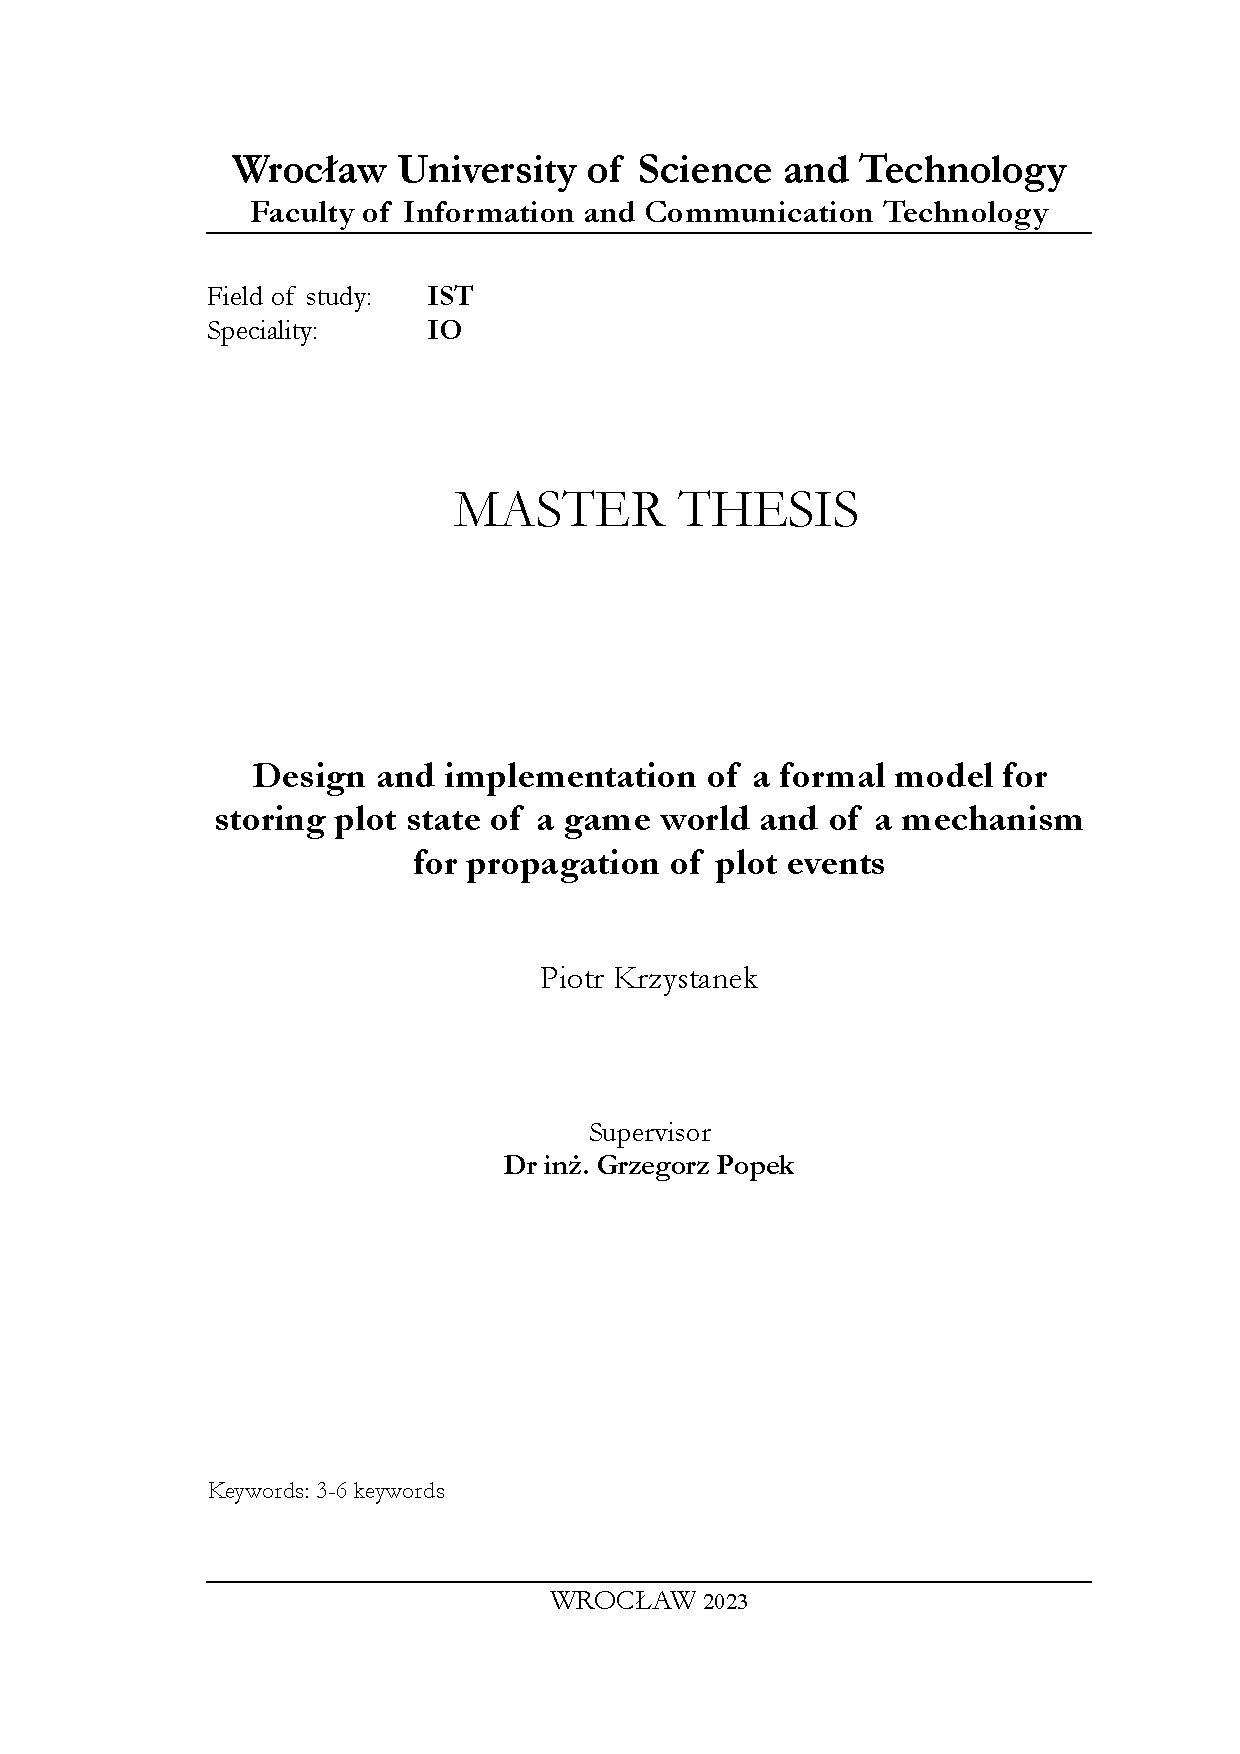
\includepdf[pages={1}]{title_page/pd_mgr_en.pdf}
\doublepage
% Add table of contents
\pagestyle{tableOfContentStyle}
% Add abstract
\pagenumbering{Roman}
\section*{Streszczenie}

Niniejsza praca magisterska bada zastosowanie systemu wieloagentowego z architekturą kognitywną do reprezentacji stanu fabularnego oraz symulacji propagacji wydarzeń fabularnych. Stan fabularny świata wraz z jego wydarzeniami jest reprezentowany przez rozproszony system agentów, z których każdy ma wiedzę o wybranych wydarzeniach fabularnych. Tradycyjne zachowanie oparte na skryptach wymaga obszernego ręcznego skryptowania dla każdej interakcji, co czyni je uciążliwym i ograniczającym w radzeniu sobie z różnymi sytuacjami. Z kolei zachowanie emergentne pozwala na bardziej dynamiczne i świadome kontekstu reakcje. Badania te wykorzystują system wieloagentowy do symulacji poszczególnych agentów z ich własnymi zachowaniami, rozszerzonymi przez zastosowanie architektury kognitywnej. Celem niniejszej pracy jest wdrożenie i opisanie systemu wieloagentowego wykorzystującego architekturę kognitywną oraz porównanie jego skuteczności z modelem epidemiologicznym wykorzystanym jako model propagacji informacji.

\section*{Abstract}

This master thesis explores the application of a multi-agent system with a cognitive architecture for representation of plot state and simulation of propagation of plot events. The plot state is represented using a distributed system of agents in which each agent has possession of chosen plot events. Traditional scripted behavior requires extensive manual scripting for each interaction, making it cumbersome and limiting in handling diverse situations. In contrast, emergent behavior allows for more dynamic and context-aware reactions. This research leverages a multi-agent system to simulate individual agents with their own behaviors, facilitated by a cognitive architecture. The objectives of this thesis are to implement and describe a multi-agent system using a cognitive architecture and compare its effectiveness with an epidemiological model used as an information propagation model.
\doublepage
\tableofcontents
\doublepage
% Set page style 
\pagestyle{custom}
\mainmatter

% Create chapters:
\Chapter{Introduction}\label{chapter:introduction}
% Start with stories
Since ancient times humans loved stories.
Some stories describe historical events, others are works of fiction.
Some inspire and teach, others let one escape from hardships of day-to-day life.
All stories have one thing in common.
One thing differentiates them from other written forms.
That thing is the existence of a plot.
% Define plot
Plot is an organized collection of events (usually in chronological order).
A plot can be realistic, based in history or it can be entirely made up.
It can be said that it is the plot that makes the story.
It brings together all the characters, their actions and thoughts as well as events within the story.

% How were stories told
Before people invented the first writing system stories were being told mouth-to-mouth.
Oral traditions continued even during the era of the written word.
Most people have heard the tales of Odysseus and his epic journey.
It is commonly attributed to the ancient poet Homer.
His work inspired both ancient and contemporary historians\cite{marincola2007odysseus}.
% Books and language
After writing got popular among common folk, the spread of storytelling in its written form took off.
In the current day, anyone can write and share the fruits of one's creative imagination with the rest of the world.
Even languages are becoming less of a barrier as not only a large portion of the population speaks English but translation technology and globalization make intercultural and international communication easier than ever\cite{coulmas1987speak}.
But writing itself is not the only way to tell a story.

% Theater
Going back to ancient Greeks, one can find the wealth of plays written to be performed on stage in the first theaters or, more precisely, amphitheaters.
Actors on stage wore masks that obscured their real faces and instead displayed a chosen emotion.
This allowed the people watching from the far seats to still understand the scene.
The aim of these performances was called catharsis\cite{hart2010art}.
Soon, the theater as is known today became born and people have been writing plays for a multitude of reasons.
% Painting
% Radio
% Cinema
% Television
% Diversity of representation in media
Books, plays, television and radio are all passive forms of media where content can be consumed by everyone in the same way.
People are diverse in their appearance, ideologies, beliefs and behaviors.
There are many groups of people with different cultures, history and traditions.
One of the main problems with what is commonly known as mainstream media (that is media that is most popular) is that it caters to the majority of its consumers.
In the old days when writing was expensive the common people could not access any books and much less find their representation in them.
Even among the people belonging to the same culture, there are many tastes and opinions.
% Interactive storytelling
People like to engage in the stories they consume and the easiest way to achieve deeper engagement is through the ability to influence the direction of the story itself.
Authors such as Chris Crawford\cite{crawford2013interactive} have written about interactive storytelling in the context of current day computer games but the concept itself is really much older than that.
In 1930 Doris Webster and Mary Alden Hopkins wrote a book titled "Consider the Consequences!".
According to the authors the book had multiple endings which depended on the "taste of the individual reader" \cite{webster1930consequences}.
These game books as they have been named (these days also referred to as "Choose Your Own Adventure" type stories\cite{kraft1981cyoa}) have evolved alongside tabletop roleplaying games.
One notable example of the genre is "Dungeons and Dragons", a game of which many people have heard even if they have not played it themselves \cite{gygax1974dungeons}.
In the current day, the genre is very diverse and consists of a multitude of games, some commercially available, others entirely fan-made.

%
This shows that interactive storytelling is a unique way of engaging and captivating audiences by allowing them to actively participate in the story.
In this form of storytelling, the audience is not just passive listeners, but active participants who are given the opportunity to make choices and influence the direction of the narrative.
Interactive storytelling increases audience engagement and immersion in the story. When the audience becomes part of the narrative, they develop a sense of ownership and become more invested in the story.
This level of immersion can lead to a more meaningful and memorable experience.
Interactive storytelling allows the audience to step into the shoes of the characters in the story and experience their emotions and decisions.
This can foster empathy and a deeper understanding of different perspectives and experiences.
By participating in the story, the audience can better appreciate the complexity of the characters' motives and actions.
Interactive storytelling can be personalized to the audience's interests and preferences.
By offering choices and different paths, the audience can tailor the story to their liking.
This level of personalization can increase engagement and create a more satisfying experience.
Interactive storytelling can encourage creativity and imagination.
By allowing the audience to make choices and shape the story, they are given a sense of agency and control.
This can inspire them to explore different paths and possibilities, leading to a more creative and imaginative experience.
In conclusion, interactive storytelling has several benefits, including enhancing engagement and immersion, fostering empathy, enhancing learning, offering personalization, increasing retention and recall, and enhancing creativity.
Interactive storytelling can be a powerful tool for creating memorable and impactful experiences for audiences of all ages and backgrounds.
%

Especially in the case of aforementioned tabletop roleplaying games, the players have nearly infinite freedom of expression and ability to influence the world limited only by their creativity.
This works only because the world exists in the minds of the players and all interactions can be simulated in the head of the player acting as the game master (a person responsible for coordinating the players actions and telling the interactive story).

The advent of computer games brought unparalleled ability for artists to allow others to become immersed in their fictional worlds.
Current advances in computer graphics make it possible to display life-like images of the game world.
No longer does a player need to rely solely on their imagination to be able to immersive themselves in the story.
While this comes with many benefits, the major downside is that the freedom to interact with the game is limited by what the developers of the game have foreseen.
Linear stories akin to movies are simple to develop while large scale open-world games are difficult.
Because of that, many games offer very shallow mechanics of interaction.
The choices that are offered to the player are often of no consequence and only exist to create an illusion that will deepen the player's engagement and immersion.

One particular example of this is the ability to break the law of the simulated world.
A player may choose to steal an apple from a market stall and usually a bunch of city guards will take pursuit.
This situation illustrates the consequence of the action undertaken by the player.
This illusion breaks however when the player was never seen stealing and then travels half the continent and tries to sell it just to be told that the vendor will not accept stolen goods.
Simplifications made in the simulation of game worlds are necessary and dictated by hardware limitations.
The same holds for choices made by the player during the game.
If a major political figure is taken captive the player may make a choice to free them and earn their trust or allow the bandits to keep them incarcerated.
Such a choice should affect the rest of the world and its impact should be growing stronger as time passes to eventually die out.
In reality however, most games do not feature such a complex interaction system.
There are exceptions to this such as "The Witcher 3" or "Fallout 2" which allows the player to influence the state of the world by making decisions in certain points of the game \cite{vickery2018directing}.
Even then, the narrative in such games always follows one of the predetermined branches.
% Interactive media
% lepsze utożsamianie się z bohaterem, możliwość kszatłtowania historii, w momencie gdy mamy wpływ, stajemy się bohaterem
% reprezentacja grup społecznych
% dopamina - osiągnięcia bohaterów stają się naszymi
% potrzeba tworzenia sztuki i opowiadania historii, na piramidzie potrzeb jest potrzeba samorealizacji, w tym tworzenia
% Games
% Information

People experience reality through the lens of their accumulated experience.
Each event in the life of a person adds another perspective on any following event.
Our behaviors are dictated by the way we perceive reality.
That perception is a combination of external sensory information and internal state of mind.
Our emotions, values and beliefs can fundamentally change the interpretation of any given situation.
As we grow old we look back on the choices we made and judge them by the standards of the present.
This simple fact means that there is no objectivity in how humans perceive reality.
Some situations or statements are simply more common in interpretation that others and thus we call them facts.
Others we refer to as opinions and some can be called delusions.

In games, the player is often tasked with accomplishing a goal which puts the future of the world at stake.
The choices made by the player should feel impactful to the overall narrative or the player will feel disengaged from the story, breaking immersion.
Often, choices can be morally ambiguous and the player should face the consequences of their actions in one way or another.
In society crimes are punishable on the basis of proof.
Proof is knowledge backed up by evidence, ergo a type of transferrable information.
An eyewitness of a crime can be untrustworthy and thus a crime might not be punished.

Within a simplified game world this mechanism is often simplified and a crime is detected and unfortunately propagated across all the land if the player is briefly witnessed even by a single person.
The same goes for other player choices and game events.
People start referencing in-game events in dialogues instantly after they happen as if seemingly everyone became aware of them instantaneously.
This can break immersion and player expectations.

Designers can not foresee all the possible actions that a player can wish to perform and thus it is not viable to write a scripted reaction to every potential choice the player makes.
That is, if the number of choices is not small enough that the player will quickly explore all possible interactions.
In order to prevent breaking the immersion of the player and maintain a believable virtual world, all simulated characters need to be independent and believable themselves.

\section*{Problem Statement}
\addcontentsline{toc}{section}{Problem Statement}

Scripted behavior is deterministic and tailored to a specific situation.
The more situations a character needs to react to, the more work is needed for scripting each interaction individually.
Generalizations of behavior help in this instance as some situations can be handled in a general way such as a character getting hurt and fleeing or fighting.
Others are more subtle and require careful scripting work to be believable and engaging.

Instead of relying on scripting and handling every possible situation via a predefined reaction, the concept of emergent behavior can be used.
The individual interactions that can be represented in a game still need to be manually scripted but the overall behavior of both single agents as well as whole groups of agents will emerge naturally.
In order for emergent behavior to be possible, an entity exhibiting it needs to be independent and aware of the context in which it exists.
For this reason a multi-agent system is used to simulate each virtual character as a separate agent with their own behaviors facilitated by a cognitive architecture.

Each agent can be said to possess the knowledge about some plot events.
The behaviors of all agents form the combined plot state of the game world.

% The main topic of research in this thesis is the applicability of a multi-agent system with cognitive architecture in implementation and simulation of an epidemiological compartmental model simulating the propagation of information.
The main goal of the thesis is design and implementation of an plot event propagation model in games.
For this reason a multi-agent system is used.
Each agent is implemented using cognitive architecture.
The plot propagation is simulated using an epidemiological model interpreted in terms of information propagation.

% Propagation of knowledge or in general information is often too simplified in games.
% Player actions should generate information that can be perceived, interpreted and propagated naturally by the other agents in the simulated game world.
% Interpretation of received (objective) information produces (subjective) knowledge.
% The distinction allows for effects such as misinterpretation and thus propagation of false information in the system.
% This can lead to interesting mechanics and interactions that simulate reality more closly, increasing player engagement and immersion.
% The main topic of research of this thesis is analysis of the three aspects of information in a game world, namely:

% \begin{description}
%     \item[perception] how, what and when information is received
%     \item[interpretation] how information becomes knowledge
%     \item[propagation] how knowledge becomes information and propagates to other people
% \end{description}

% The analysis as well as simulations and other research takes into account the overall end goal of the thesis being implementation in games where computing power is limited and real-time performance is paramount.
% In a world with access to information in real-time across the globe via the use of internet, all models will be inherently different in comparison to a world without any such technology.
% This thesis takes into account medieval style worlds with fantasy elements such as magic or mythical creatures but no advanced communication techniques.

\section*{Thesis Objectives}
\addcontentsline{toc}{section}{Thesis Objectives}

The objectives of this thesis include the design and implementation of a formal model for storing plot state of a game world and of a mechanism for propagation of plot events.
It is actually argued that instead of a centralized model trying to handle plot events' propagation, it can be attained as an emergent property of a multi-agent system.
The agents possess knowledge about the state of the plot and by interacting with each other cause propagation of plot events.
To facilitate the agent's complex behavior, cognitive architecture is used.
For the simulation of plot event propagation an epidemiological compartmental model is used.
The implementation of the multi-agent system is compared with the epidemiological model.
The title of the thesis refers to plot state and plot events.
The plot state is understood as the state of the population, divided into the compartments defined by the chosen epidemiological model.
The plot event is the act of an an agent transferring the information (infecting) another agent.
The thesis aims to answer the following Research Questions:

\begin{description}
    \item[RQ1] Can a solution using a multi-agent system with cognitive architecture be used in a game to simulate plot event propagation?
    \item[RQ2] Are the resulting information propagation dynamics consistent with the dynamics of the epidemiological model?
\end{description}

% To properly understand the three aspects of information previously mentioned, the distinction between information and knowledge needs to be made.
% Information itself needs to be defined as well.
% To model the behaviour of different models, a cellular automata approach is chosen.

\section*{Thesis Outline}
\addcontentsline{toc}{section}{Thesis Outline}

The thesis is divided into $5$ chapters.
Related works are described in chapter \ref{chapter:related}.
Chapter \ref{chapter:chapter1} describes the multi-agent systems and various chosen cognitive architectures.
The chosen architecture is implemented and described in chapter \ref{chapter:chapter2}.
In this chapter experiments and their results are also described.
Lastly, chapter \ref{chapter:conclusions} contains conclusions and ideas for future work.

% Zarysuj strukturę swojej pracy dyplomowej.
% Ogólnie przedstawienie pracy.

% Przykładowo:

% ,,Praca dzieli się na $7$ rozdziałów (\dots)''.
% Rozdział \ref{chapter:politechnika} dotyczy (\dots). T
% emat został rozwinięty~w~\ref{chapter:podrozdzial}.
\Chapter{Related Work}\label{chapter:related}

In 1989, Ackoff\cite{ackoff1989data} defined the hierarchy of the human mind as consisting of wisdom at the very top and descending into understanding, knowledge, information and further into data.
The more popularized variant of this hierarchy being DIKW (data, information, knowledge, wisdom), became widespread in literature regarding knowledge management\cite{skyrme2007knowledge}.
According to Liew\cite{liew2013dikiw} trying to accurately define data, information and knowdlege will result in circular definition.
To solve that problem he proposes a DIKIW model where "I" stands for "Intelligence".
Irrespective of chosen framework, everyone agrees that information and knowledge are related but represent different levels of abstraction.
While data is raw and unprocessed before it can become information, similarly information needs to be retained and assimilated to become knowledge.
The scope of this thesis covers only information understood as statements of fact and knowledge defined as retained and processed information.

A population of people can be said to possess knowledge similarly to a single individual.
Often a crowd has greater knowledge than any individual.
Surowiecki said "under the right circumstances, groups are remarkably intelligent, and are often smarter than the smartest people among them"\cite{surowiecki2005wisdom}.
To understand how knowledge is gained within a population one should analyze the way information itself is propagated.
In fact, people have already noticed that certain facts, stories or news share similarities with viral infections in how they spread across the whole population and eventually die out.
One such example is the work done by Liu et al.\cite{liu2016} where the authors describe how information spread can be explained using epidemiological models.
Truly, the simplest of such models called SIR\cite{weiss2013sir} can be used to describe in simple terms how a population can be partitioned into groups of \emph{Susceptible} (people who haven't encountered the viral information yet), \emph{Infected} (those who know the news and are willing to share it) and \emph{Removed} (everyone who either lost interest or simply never exhibited it).
There are however differences between infectious diseases and information.
For this reason variations of the SIR model became born.
Zhao et al.\cite{zhao2012sihr} have developed the SIHR model where H stands for \emph{Hibernators}.
The authors stress the importance of forgetting and remembering in trying to model the spread of information.
Another variation worth noting is the SCIR model consisting of \emph{Susceptible}, \emph{Contacted}, \emph{Infected} and \emph{Refractory}\cite{xiong2012scir}.
Both models use complex systems in order to simulate information propagation.
Other attempts at modelling information propagation are networks\cite{rodriguez2013} and cellular automata\cite{silva2020}.
Most literature dealing with the topic refers to social media, blogs and internet as the main medium of information exchange.
Relatively few works analyze the mechanisms behind word-of-mouth communication.
In 2003 at the "Symposium on Applications and the Internet", Takeuchi, S. and Kamahara, J. and Shimojo, S. and Miyahara, H. have presented their work titled "Human-network-based filtering: the information propagation model based on word-of-mouth communication" which deals with simulating how certain information is spread based on the filters of interest\cite{takeuchi1183031}.
Most authors treat knowledge of information as a binary value.
In reality the level of knowledge is often more complicated.
Silva et al.\cite{silva2020} propose the application of cellular automata to model information expressed as a linear value.

\Chapter{Represenation of plot state using a agent-based simulation}

\section{Agents and architecture}

Both the player and any non-playable characters can be called agents.
Each agent is independent from the rest and is able to act based on the subset of the plot available to them.
The actual implementation of each agent's behaviour can be as simple as a hardcoded line of dialogue and as complex as a set of rules enabling emergent behaviour.
General plot of the game as experienced by the player is the sum of interactions and sub-plots of the individual agents in the game.
Grey et al.\cite{grey2011procedural} proposed a solution using agent-based simulation to create procedural quests.
This work focuses on extension of the original approach using a SOAR cognitive architecture\cite{rosenbloom1993soar}.

\subsection{SOAR}

One of the most important developments in the area of multi-agent systems and cognitive modelling was the SOAR (State, Operator, And Representation) cognitive architecture \cite{laird2019soar}.
It is a cognitive architecture that is designed to simulate human thinking and problem-solving processes.
At its core, SOAR is a symbolic, production-based system that uses rules to guide behavior.
This architecture consists of two major components:

\begin{itemize}
    \item Procedural memory (production memory) - set of production rules that can modify the state of the world and by extension, the state of the working memory by proposing operators
    \item Working memory - fact based knowledge represented by a symbolic graph structure describing the current state of the world
\end{itemize}

Many implementations of this architecture additionally include the concept of long-term memory structure that accumulates knowledge during the whole lifetime of the agent.
In general, implementation of the SOAR architecture can be called a production system.
Unlike many traditional production systems however, all rules that match against the current state of the world will fire (execute actions) in parallel.
This means that the list of rules is not ordered and conflicting operators may be proposed.
In such cases the usual strategy is to create a substate of the working memory with a new goal of conflict resolution.

The SOAR architecture has been successfuly utilized in creation of video game AI agents.
Examples include the application of this architecture to create an autonomous agent designed for playing Quake\cite{laird2001knows}, StarCraft\cite{turner2013soar-sc} and Descent 3\cite{van1999developing}.
Michael van Lent and John Laird in their work "Developing an Artificial Intelligence Engine"\cite{van1999developing} describe a decision cycle in an inference machine:

\begin{itemize}
    \item Perceive: Accept sensor information from the game
    \item Think: Select and execute relevant knowledge
    \item Act: Execute actions in the game
\end{itemize}

This cycle combined with the SOAR architecture allows for creation of a versatile agent capable of processing and propagating plot events in the game.
The first step allows the agent to modify the state of the working memory.
It can detect visible objects, including other agents and interactables such as containers, doors or even writings.
Then, the second step uses the working memory combined with production rules (procedural memory) to propose operators to execute.
Operators modify the state of the world, for example by moving the agent, taking the contents of a container, opening doors or interacting with another agent.
This constitutes the last step of the cycle and allows the agent to go back to the first step and update its working memory in preparation for the next step.

This architecture is versatile in that it can be used to model even very complex behaviours.
In order to avoid conflicts in the proposed operators by production rules that try to solve different goals, a goal token can be inserted into the working memory and used as a dependency in the production rules.
This way an agent may have a rule that changes the goal of the agent and thus modifies its next sequence of actions.

\subsection{Perceive}

The agent is equipped with simulated sensors that feed into its working memory.
These sensors interact with the simulated world and process the description of the world producing information that is then stored in the working memory of the agent.
Sensory information might include sight, hearing, sense of smell and other commonly thought of senses as well as abstract and arbitrary information that the agent can somehow perceive.
The combined information from all the sensors might produce information regarding the agent's awareness of the vicinity and the location of other agents in the simulated system as well as the state of the agent's body and own position in the game world.
The information is presented to the agent and it is up to the agent to decide what to do with it.
Sensors may only influence working memory of the agent.

\subsection{Think}

Agents have procedural memory that is represented by a collection of production rules that are executed in parallel.
Each rule might take as input an arbitrary set of working memory elements (WME), check arbitrary preconditions and produce arbitrary operators that when evaluated will change the state of the simulated world by means the agent's action.
While working memory is perfect for storing the immediate description of the agent's state, it is perhaps ill suited for storage of event based information elements.
For this reason the notion of long term memory is used for storage of facts characterized by timestamp of occurrence and description of the event.
Procedural memory and production rules therein may also utilize this storage to work with temporal data, for example to facilitate the agent remembering its travel trajectory or recording events such as successful executions of certain actions.
Procedural memory is usually immutable after creation of the agent but it is possible to store a production rule inside of working memory and by means of another production rule, modify the procedural memory adding the new rule to the bank of rules the agent possesses.
This can simulate agent learning new inference rules and behaviours, for example through reading a book or being taught by other agent.

\subsection{Act}

The act of action when performed by the simulated agent is represented by an operator being evaluated.
An operator represents an action that an agent wishes to perform.
The game world is in charge of evaluating the results of the operator and rejecting it in case the agent is not allowed to perform it due to any condition that the agent itself is not aware of.
Because production rules are executed in parallel and thus output multiple operators, it is possible for conflicts to occur.
A single agent may think to move forward and back at the same time.
Because the order in which actions are performed may impact the result, it is important to define a conflict resolution strategy, either for each agent or for the whole game in general.
Such a strategy does not need to necessarily be deterministic as usually it is impossible to determine which operator should take precedence and defining conflict resolution policies for each possible set of conflicting operators is often not a viable approach.
One example of a conflict resolution strategy is a strategy that chooses a random order for conflicting operators and executes them until one is accepted.
This shows the second part of the problem which is conflict detection.
Any two operators can be conflicting in terms of resulting state of the game world.
The simplest approach is not allowing the agent to execute multiple operators at the same time and instead force it to choose one specific action instead.

\subsection{Interactions}

An agent might lack the sense of vision and instead start with its known position WME at coordinates $v_0=(0, 0)$.
It wishes to progress forward (positive $y$ axis) and so proposes the operator $Move(Agent, 0, 1)$ via a production rule with constant output.
The game world accepts the operator, evaluates it and the agent is then made aware of the operator's successful execution.
The agent now has the position WME set to $v=(0, 1)$.
It proposes the same operator again.
This time the game world rejects the action because of a wall that stands at $v=(0, 2)$.
The agent did not modify its position WME this time but added a second WME $WallAt(0, 2)$.
A production rule exists that checks if there is a $WallAt$ WME directly ahead of the current position and if so, produces operator $Move(Agent, 1, 0)$.
The production rule that produces the constant $Move(Agent, 0, 1)$ operator fires as well and afterwards the agent needs to decide which action to take.
The agent has a conflict resolution strategy defined as:

\begin{itemize}
    \item choose random
    \item fallback when action rejected
\end{itemize}

This policy means that either the lateral move will be selected by random chance or the previous operator will be selected, evaluated, subsequently rejected and a fallback would occurr to the next one.
This example shows that a virtual agent possesses a limited capacity to learn and build the information bank describing the state of the world around it.
In some implementations, the immediate position of the agent would be stored as WME while the position of each discovered wall would be put in long-term memory.

\subsection{Simulation constraints and limitations}

The simulatated environment presented in this work was designed to resemble the environment described by Grey et al.\cite{grey2011procedural} which in turn used the implementation done by Prageeth Silva\cite{silva2010shadow}.
As of the time of writing, the original implementation of Shadow Quest used in evaluation of Grey's model is unavailable and so a custom implementation with modifications was made specifically for the sake of experimentation.
Each agent may occupy a single tile in a grid-based world.
The temporal structure used in the design of the simulation is based on the concept of turns.
Because the interaction with a human player is not necessary to simulate the progression of a procedurally emergent plot, the turns are simply simulatin steps.
Within a single turn all agents execute the aforementioned decision cycle, starting from receiving information regarding the state of the world around them, deciding on the action to perform and finally executing it.
The simulation used for evaluation of the model presented in this work is limited to a set of actions that each agent may perform.

\begin{itemize}
    \item Idle - agent does nothing, stays idle for the whole turn
    \item Move - agent may decide to move in one of the four cardinal directions by a single tile
\end{itemize}

Because all agents execute their actions concurrently, conflicts may occur which the simulation engine must resolve.
For the sake of simplicity, a simple conflict resolution strategy was chosen where a random agent takes priority.
The second agent is overriden to have been idle for that turn.

% \section{Evaluation scenarios}

% \subsection{Scenario 1}

% The player is tasked with solving a murder mystery in a closed space.
% The gameplay loop consists of talking with non-playable characters and collecting clues.
% There are three suspects, labeled A, B and C respectively.
% The player must first obtain the first clue related to the weapon used by investigating the scene.
% Then, during interviews they should obtain the clues relating to who possesses the weapon and who has a motive.
% After that, the player might make an accusation and win the game.

% In this scenario the player and characters are independent agents.
% The scene is a special object that can be interacted with to gain the first clue.
% The communication happens only between each character and the player and is uni-directional.
% The list of possible clues is predefined.

% \subsection{Scenario 2}

% The player is tasked by a stall owner to steal a ring from the jewelery stall and plant it in another seller's pocket.
% After the player does so, the stall owner yells for the guards to come arrest the thief.
% If the ring is in the other seller's pocket, that seller will be considered the culprit and arrested.

% In this scenario the player is able to interact with the task giver, the jeweler and the seller being framed.
% The plot depends on the choices the player makes and the order they make them in.
% If the player never plants the ring, the task giver will be punished for false accusation and will instead accuse the player.
% If the player plants the ring in the pocket of the task giver, they will be the one arrested instead.
% On the other hand, leaving the ring untouched and reporting to the task giver will cause the task giver to not be taken seriously as the jeweler will deny any theft taking place.

% \subsection{Scenario 3}

% The player overheard the general of enemy army talking about the plan to invade in three days.
% They must reach the capital and inform the king of the danger to prepare the defensive.

% This scenario is time sensitive and shows example of uni-directional interaction between the player and the enemy general.

% \subsection{Scenario 4}

% A dragon is seen flying from the mountains towards the forest.
% The player is tasked with tracking it down.

% Depending on where the player starts, they might or might not have witnessed the dragon themselves.
% Through talking with the non-playable characters the player may find out who was a witness and who only heard about the dragon.
% Based on the time of sighting, the player may deduce the direction of the dragon's flight.

\Chapter{Conclusions and Future}\label{chapter:conclusions}

The thesis contains description of the solution for implementation of an epidemiological compartmental model using a multi-agent system with the SOAR cognitive architecture.
Epidemiological models have application in information propagation as described previously and so they can be used to model how information travels across a population based on a set of parameters such as the rate of spread.
The results show visible correlation between the mathematical representation of the SIR model and the data obtained from the simulation of the multi-agent system.
This means that games could utilize multi-agent systems and a cognitive architecture such as SOAR to obtain immersive simulation of each agent.
The main benefit of the adapted architecture was the composability of the behavior rules which enabled emergent behaviour as opposed to a hierarchical description of decision trees and other similar approaches.

\section{Conclusions}

In the thesis objectives three research questions have been proposed.
The experimentation and research done during the writing of this thesis lead to the following answers to each of the research questions:

\begin{description}
    \item[RQ1] Can a multi-agent system display emergent behaviour?
    \item[] A multi-agent system can display emergent behavior by composing simple behavior rules, for example using a cognitive architecture such as SOAR, described in this thesis.
    \item[RQ2] Can an epidemiological compartmental model be simulated using a mutli-agent system with a cognitive architecture?
    \item[] Epidemiological compartmental models such as SIR have shown to be possible to simulate with the application of SOAR cognitive architecture. Figures \ref{fig:experiment4-diagrams} and \ref{fig:experiment1-diagrams} clearly show the ability of the proposed solution to match the output the SIR model.
    \item[RQ3] Can a solution using a multi-agent system with cognitive architecture be used in a game to simulate information propagation?
    \item[] As described previously, many authors successfuly use compartmental epidemiological models to simulate information propagation. Because the presented solution is capable of simulating a SIR model, it can be used to likewise simulate information propagation in a game where each virtual character is an independent agent.
\end{description}

\section{Future work}

It can be seen that the potential of the adapted architecture is still unexplored in full.
The area of emergent behavior in multi-agent systems is wide and this thesis analyses only the aspect related to propagation of information among a population of agents.
One aspect that was out of the scope of this thesis was performance considerations of the implementation of the described architecture.
For this reason future work could be related to stress testing of the approach and analysis of implementation techniques used to improve the viability of adaption of this solution in games where performance concerns stem from the scale of the simulated world and the complexity of desirable agent behaviour.
Additionally, research related to modelling of scripted behaviour as a set of independent behaviour rules could be done to facilitate transition from scripted to emergent behaviour.

In game design relying solely on emergent behaviour might prove to be difficult when the designer wishes to express a certain complicated sequence of events which might be hard to define in terms of behaviour and inference rules.
In that case it is possible to define a special working memory element called $ScriptSequence_N$ where $N$ is the stage of execution, meaning that the agent which is about to execute the scripted sequence of actions will have the WME $ScriptSequence_0$.
Then, a general guard clause should be built in all the behaviour and inference rules to avoid execution if any WME present is prefixed with $ScriptSequence$.
Finally, each step of the scripted sequence should be defined as a behavior rule that executed if the $ScriptSequence_N$ matches with the step of the script expressed by said rule.
The $OnSuccess$ callback should be then used to modify the state of the working memory and advance the sequence by one.
This makes it possible to embed scripted behaviours in an otherwise emergent behaviour based system of agents.

One can identify two kinds scripted behaviours.
The first kind are static scripts which assume the state of the world to be known and constant at the moment of execution.
These could be used to orchestrate cut-scenes and enable cinametic behaviour to be embedded in the game.
The second kind are behaviour sequences which are simply complex behaviour patterns that are spread across many simulation steps.
Behaviour patterns are human designed patterns of behaviour as opposed to emergent patterns.
This kind of scripts should take into consideration the possibility of failure at any moment as the state of the world when such a sequence is triggered is not necessarily known and thus it may be that a proposed operator will fail and be rejected.
In such a case it is up to the designer to determine whether an alternative path should be taken or the sequence should be abandoned altogether.

In general, scripted sequences are an important aspect of any game and the ability to express them within the constraints of the proposed solution is necessary for it to be considered a viable option to be used in any real game.
Thus, work can be done in this aspect to determine how an emergent behaviour based solution can be used to easily express arbitrary scripted sequences of actions.

In conclusion, the proposed approach exhibits potential for usage in game development but also great complexity and a new set of challenges that are yet to be solved.
% Redefine plain for 1st bibliography page style
\resetformatting
% Please read :
%https://www.overleaf.com/learn/latex/Bibliography_management_with_bibtex
\pagestyle{bibliographyStyle}
\bibliographystyle{abbrv}
\bibliography{bibliography}

% Add list of figures and tables
\pagestyle{custom}
\newpage
\pagestyle{ListofFiguresStyle}
\listoffigures
\newpage
\pagestyle{ListofTablesStyle}
\listoftables
\end{document}